This section contains all software requirements both functional and non-functional.
A requirement has the following properties:
\begin{itemize}
	\item[\bf{ID}] Uniquely identifies requirement within all TaskList documents.
	\item[\bf{Title}] Gives the requirement a symbolic name.
	\item[\bf{Description}] The definition of the requirement.
	\item[\bf{Priority}] Defines the order in which the requirements should be implemented. Priorities are designated from highest to lowest.
	Possible values are 1 (first to implement), 2 and 3 (last to implement).
	\item[\bf{Risk}] Specifies risk of not implementing this requirement. It shows how the particular requirement is critical to the system.
	there are the following risks levels and associated impact to the system if the requirement is not implemented or implemented incorrectly.
		\begin{itemize}
			\item {\bf Critical (C)}  will break the main functionality of the system. The system can not be used if this requirement is not implemented.
			\item {\bf High (H)} will impact the main functionality of the system. Some function of the system could be inaccessible, but the 
			system can be generally used.
			\item {\bf Medium (M)} will impact some systems features, but not the main functionality. System can be used with some limitation.
			\item {\bf Low (L)} the system can be used without limitation, but with some workarounds.

		\end{itemize}

  \end{itemize}


\subsection{Functional Requirements}
\label{requirements:functional}

\begin{requirement}{Introducing Tasks}
	\label{requirements:functional:tasks}
    \desc{The system shall provide the user with the capability of adding a Task in Tomboy Notes.}
    \priority{1}
    \riskref{C}
\end{requirement}

\begin{requirement}{Grouping Tasks together}
	\label{requirements:functional:grouping_tasks}
    \desc{The system shall provide the user with the possibility to group certain tasks together in a list called a task list.}
    \priority{1}
    \riskref{C}
\end{requirement}

\begin{requirement}{Priorities for Tasks}
	\label{requirements:functional:task_priority}
    \desc{The user can optionally add priorities to individual tasks and task lists.}
    \priority{1}
    \riskref{H}
\end{requirement}

\begin{requirement}{Due Dates for Tasks}
	\label{requirements:functional:task_due_date}
    \desc{The user can optionally add due dates to individual tasks and task lists.}
    \priority{1}
    \riskref{H}
\end{requirement}

% TODO make this according to our issue discussion
\begin{requirement}{Subtasks}
	\label{requirements:functional:subtask}
    \desc{The system provides the user with the ability to model a task as a complex task consisting of possibly multiple subtasks.}
    \priority{1}
    \riskref{H}
\end{requirement}

\begin{requirement}{Exporting Tasks}
  \label{requirements:functional:export}
  \desc{The system provides a function to export all tasks in all notes and their corresponding information in the ICAL \ref{ical} format.}
  \priority{3}
  \riskref{L}
\end{requirement}


    \subsubsection{Entity Diagram}
    The following diagram shows all defined entities from the requirements above and their relations.
    As we can see a Task is basically modeled as a string and - if its a more complex task - can link to other notes.
    \begin{figure}[h]
	    \centering
        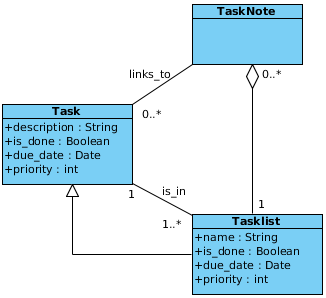
\includegraphics[width=0.5\textwidth]{graphics/entity_diagram.png}
        \caption{TaskList entities and relations}
        \label{entities_relations}
    \end{figure}
    
    This diagram does not define classes that must be implemented in software, but just the common entities



    \subsubsection{User Interface}
    \label{requirements:interfaces:user}

    \begin{requirement}{Create Task List}
    \label{requirements:interfaces:user:create_tasklist}
      \desc{The user shall be able to create a new task list with a button or a shortcut text, like ``[]''. These lists expand automatically and contain individual tasks that can be marked as done.}
      \priority{1}
      \riskref{C}
    \end{requirement}

    \begin{requirement}{Edit Task List}
    \label{requirements:interfaces:user:edit_tasklist}
      \desc{The user can add, remove and change single task list items by directly editing the task list in the note itself.
			A task description can be edited by directly editing the text. Setting the due date, priority and done flag will be realized through embedded GTK\# widgets. A task will be removed automatically from the task list if the user deletes the text describing the task and the corresponding line in the editor. A task list will be removed if there are no more tasks in the list.}
      \priority{1}
      \riskref{H}
    \end{requirement}
 
    \begin{requirement}{Setting a Due date}
      \label{requirements:interfaces:user:due_date:set}
      \desc{The user is able to set a due date for a single task or an entire task list by adding a widget for the due date over a menu button and/or a shortcut text. The Widget will be located somwhere next to the task/task list.}
      \priority{2}
      \riskref{M}
    \end{requirement}

    \begin{requirement}{Due date visualization}
      \label{requirements:interfaces:user:due_date}
      \desc{The system shall visualize the due date (if set) to the user. It will, based on the current date, change the text color of the date: If it is
      far in the future it will be green, if the day is in near future or even in the past the text color will be red.}
      \priority{2}
      \riskref{M}
    \end{requirement}

    \begin{requirement}{Set Priority}
      \label{requirements:interfaces:user:priority}
      \desc{The user is able to set a priority for a single task or an entire task list by adding a widget for the priority over a menu button and/or a shortcut text. The Widget will be located somwhere next to the task/task list.}
      \priority{2}
      \riskref{M}
    \end{requirement}

    \begin{requirement}{Priority visualization}
      \label{requirements:interfaces:user:priority}
      \desc{The system shall visualize the priority of a task by displaying the priority as a number in a text color which is unique to this particular priority.}
      \priority{2}
      \riskref{M}
    \end{requirement}

    \begin{requirement}{Create Subtasks}
      \label{requirements:interfaces:user:subtasks}
      \desc{The user can optionally create a task consisting of one or multiple other task lists considered as sub tasks for this particular task by creating hyperlinks linking to other tasks.}
      \priority{1}
      \riskref{H}
    \end{requirement}

    \begin{requirement}{Show / hide completed Tasks}
      \label{requirements:interfaces:user:show_hide}
      \desc{The user gets various possibilities to handle completed tasks. He can show them crossed out, he can hide them, and he can show them after the completed tasks. }
      \priority{2}
      \riskref{M}
    \end{requirement}

    \begin{requirement}{Reorder Task Lists}
      \label{requirements:interfaces:user:reorder}
      \desc{The user has the possibility to order the task lists according to various criteria, like due date, priority, date added etc.}
      \priority{2}
      \riskref{L}
    \end{requirement}

    \begin{requirement}{Filter Notes}
      \label{requirements:interfaces:user:filter}
      \desc{The user can query for a list of notes by setting constraints which involve searching for notes who have unfinished tasks or contain 
      tasks which are over their corresponding due date.}
      \priority{2}
      \riskref{M}
    \end{requirement}


    \subsubsection{System Interfaces}
    \label{requirements:interfaces:system}
    \begin{requirement}{Tomboy directories}
	  \label{requirements:interfaces:system:directories}
      \desc{All user data will be stored in the \textit{standard Tomboy configuration directories}\footnote{\url{http://live.gnome.org/Tomboy/Directories}}}
      \priority{1}
      \riskref{H}
    \end{requirement}


    \subsubsection{Software Interfaces}
    \label{requirements:interfaces:software}

    \begin{requirement}{Tasks Persistence}
	  \label{requirements:interfaces:software:persistence}
      \desc{All the necessary information about tasks and tasks list will be made persistent using the provided facilities by Tomboy to store note information. The XML format used by Tomboy to store notes will be extended with additional attributes as necessary to suite our needs.}
      \priority{1}
      \riskref{C}
    \end{requirement}

    \begin{requirement}{Tomboy Version}
	  \label{requirements:interfaces:software:tomboy:version}
      \desc{The addin shall be designed for Tomboy version 1.2.0. Future and past releases of Tomboy are available in the official git repository\footnote{\url{http://git.gnome.org/browse/tomboy/}}}
      \priority{1}
      \riskref{H}
    \end{requirement}


    \subsubsection{Supported Operating Systems}
    \label{requirements:os}
    \begin{requirement}{Platform independance}
      \label{requirements:os:independance}
      \desc{The Addin will work on any oerating system with a working installation of Tomboy (as defined in \ref{requirements:interfaces:software:tomboy})}
      \priority{2}
      \riskref{M}
    \end{requirement}

\subsection{Nonfunctional Requirements}
\label{requirements:nonfunctional}

    %TODO fill in
    % => Bugs, unit tests

    \subsubsection{Usability}
    \label{requirements:nonfunctional_start}
    \label{requirements:usability}
    \begin{requirement}{Default language}
      \label{requirements:usability:default_language}
      \desc{All system messages, texts, log entries and help documentation must by default be available in English.}
      \priority{1}
      \riskref{M}
    \end{requirement}

   
    \begin{requirement}{Translations}
      \label{requirements:usability:translations}
      \desc{Tomboy uses the internationalization and localization library \textit{GNU gettext}\footnote{\url{http://www.gnu.org/software/gettext/}}. 
        The Addin will integrate this built-in language support and will therefore enable anyone being capable of writing Tomboy/Gnome translations to add additional language translations to the project.}
      \priority{2}
      \riskref{M}
    \end{requirement}

    \begin{requirement}{Documentation}
      \label{requirements:usability:documentation}
      \desc{The Addin will provide an online documentation (currently available on the git, but designed to fit into the manual files of tomboy) that will list all available functionalities and enable the computer experienced user to use the all possible functionalities after reading the corresponding section}
      \priority{1}
      \riskref{M}
    \end{requirement}

    \subsubsection{Reliability}
    \label{requirements:reliability}
    \begin{requirement}{Failures}
      \label{requirements:reliability:failures}
      \desc{The project does not have any point of failure that will cause Tomboy to crash or freeze.}
      \priority{1}
      \riskref{H}
    \end{requirement}
    
    \begin{requirement}{Logging}
      \label{requirements:reliability:logging}
      \desc{The Addin provides log information about performing critical code segments and encountered errors.
        The Addin shall provide full information about failures and errors if not logged by Tomboy itself.
        This information shall include: time of failure, origin (subsystem or component) where a failure occurred, severity and description of error or failure. 
        Diagnostic information will be logged and saved in the text file tomboy.log in the standard directory for Tomboy configuration information (See \ref{requirements:interfaces:system}).}
    \end{requirement}

    \subsubsection{Performance}
    \label{requirements:performance}

    \begin{requirement}{Optimisation platform}
      %TODO: maybe merge this into system description?
      % Not even sure this is necessary but I thought need to be precise about which computers should fulfill the performance requirements
      \label{requirements:performance:optimisation}
      \desc{The optimisation platform (description of computers that will fulfill the performance requirements) is any nowadays personal computer with at least 1GB of RAM, 1.5GHz CPU and more than 30GB of hard disk with Windows (XP or newer release), Ubuntu or derivates (current (TODO: fill in current version), or Debian}
      \priority{1}
      \riskref{M}
    \end{requirement}

    \begin{requirement}{Response times}
      \label{requirements:performance:responsetime}
      \desc{The basic task operations (Introducing and grouping of tasks and adding due dates and priorities to tasks see \ref{requirements:interfaces:user}) shall not take longer than 1 second.}
      %TODO: Why 1 second
      \priority{1}
      \riskref{M}
    \end{requirement}

    \begin{requirement}{Initialising Tomboy}
      \label{requirements:performance:initialization}
      \desc{Initialising Tomboy (startup) may not take longer than twice as long as without the Addin on the platform as described in \ref{requirements:performance:optimisation}, since the splash screen is already a bit long and loading takes a while.}
      \priority{1}
      \riskref{M}
    \end{requirement}

    \subsubsection{Maintainability}
    \label{requirements:maintainability}
    %TODO: Not sure this is necessary, but it's good to mention anyway, don't you think?
    \label{requirements:maintainability:github}
    \begin{requirement}{Git repository}
      \desc{The project's source code will be available on \url{git://github.org/rggjan/Tomboy-Todo-List}}
      \priority{1}
      \riskref{M}
    \end{requirement}

    \label{requirements:maintainability:codedoc}
    %TODO: Agree on this
    \begin{requirement}
      \desc{All source code will be available in a documented version introducing XML comments as defined by the ECMA C\# standard.
      %TODO: Link
}
    \end{requirement}

    \subsubsection{Deployment}
    \label{requirements:deployment}
    \begin{requirement}{Installation from library}
      \label{requirements:deployment:installation}
      The Addin can be installed by compiling the corresponding library into the Addin directory of Tomboy (See \ref{requirements:interfaces:system}).
    \end{requirement}

    \begin{requirement}{Activation of the Addin}
      \label{requirements:deployment:activation}
      Once a working copy of the .dll from \ref{requirements:deployment} is in the corresponding directory or included into the source of the project, Tomboy will automatically detect the Addin and supply the Addin register of the preferences menu with the possibility to enable it.
    \end{requirement}

    \subsubsection{Licensing Requirements}
    \label{requirements:license}
    \begin{requirement}{license compliance}
      \label{requirements:license:compliance}
      \desc{Tomboy uses the \textit{GNU Lesser GPL} \ref{lgpl}. 
        To be consistent, the project will adapt this license for any source code.}
      \priority{1}
      \riskref{M}
    \end{requirement}


    \subsubsection{Design Constraints}
    \label{requirements:constraints}
    \begin{requirement}{Standard compliance}
      \label{requirements:constraints:standards}
      \desc{The project will be seen as part of Tomboy and will therefore comply to any existing standards and regulations imposed by Tomboy itself or the GNOME project. This will most notably include language support (\ref{requirements:usability}) and licensing (\ref{requirements:license}), but also requirements like style guidelines\footnote{\url{http://developer.gnome.org/doc/guides/programming-guidelines/index.html}} and design philosophy\footnote{\url{http://library.gnome.org/devel/hig-book/stable/}}}
      \priority{1}
      \riskref{M}
    \end{requirement}

    % => modules (textbuffer, note gui, notes window gui)
    % I don't really see this being a design constraint (constraint = Auflage/Bedingung) - Gabriel
    % OK, then put it somewhere else...

    \label{requirements:nonfunctional_end}
